% Created 2016-02-10 Wed 15:55
\documentclass[11pt]{article}
\usepackage[utf8]{inputenc}
\usepackage{lmodern}
\usepackage[T1]{fontenc}
\usepackage{fixltx2e}
\usepackage{graphicx}
\usepackage{longtable}
\usepackage{float}
\usepackage{wrapfig}
\usepackage{rotating}
\usepackage[normalem]{ulem}
\usepackage{amsmath}
\usepackage{textcomp}
\usepackage{marvosym}
\usepackage{wasysym}
\usepackage{amssymb}
\usepackage{amsmath}
\usepackage[version=3]{mhchem}
\usepackage[numbers,super,sort&compress]{natbib}
\usepackage{natmove}
\usepackage{url}
\usepackage{minted}
\usepackage{underscore}
\usepackage[linktocpage,pdfstartview=FitH,colorlinks,
linkcolor=blue,anchorcolor=blue,
citecolor=blue,filecolor=blue,menucolor=blue,urlcolor=blue]{hyperref}
\usepackage{attachfile}
\usepackage{graphicx}
\usepackage{subfigure}
\usepackage{pdfcomment}
\date{\today}
\title{blog}
\begin{document}

\section{Backend specific output}
\label{sec-1}

\begin{minted}[frame=lines,fontsize=\scriptsize,linenos]{common-lisp}
(setq org-export-babel-evaluate t)
\end{minted}

\begin{verbatim}
t
\end{verbatim}

\begin{minted}[frame=lines,fontsize=\scriptsize,linenos]{common-lisp}
org-export-current-backend
\end{minted}

\begin{verbatim}
latex
\end{verbatim}



\begin{minted}[frame=lines,fontsize=\scriptsize,linenos]{python}
import matplotlib.pyplot as plt

plt.plot([3, 4, 5, 6])

print backend

if backend == 'latex':
    plt.savefig('backend.pdf')
    print '''
#+caption: Your figure in pdf.
[[./backend.png]]'''
elif backend == 'html':
    plt.savefig('backend.png')
    print '''
#+caption: Your figure in html.
[[./backend.png]]'''
else:
    plt.show()
\end{minted}

latex

\begin{figure}[htb]
\centering
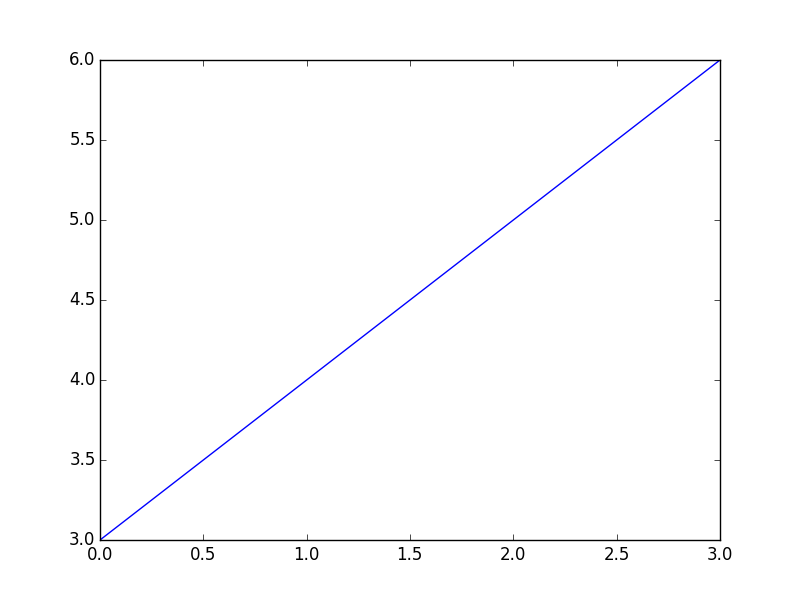
\includegraphics[width=.9\linewidth]{./backend.png}
\caption{Your figure in pdf.}
\end{figure}
% Emacs 25.1.50.1 (Org mode 8.2.10)
\end{document}